
\documentclass[journal]{IEEEtran}
\usepackage{blindtext}
\usepackage{graphicx}
\usepackage{amsthm,amsfonts,mathrsfs,amsmath}
\newtheorem{definition}{Definition}
\usepackage[T1]{fontenc}

\makeatletter
\newcommand{\pushright}[1]{\ifmeasuring@#1\else\omit$\displaystyle#1$\ignorespaces\fi}
\makeatother

%%%%%%%%%%%%%%%%%%%%%%%%%PACKAGE FOR ALGORITHMS

\usepackage{algorithm}
\usepackage{algpseudocode}
\newcommand{\Break}{\State \textbf{break} }
\algnewcommand\algorithmicforeach{\textbf{for each}}
\algdef{S}[FOR]{ForEach}[1]{\algorithmicforeach\ #1\ \algorithmicdo}
\algblockdefx[Loop]{Loop}{EndLoop}[1][]{\textbf{Loop} #1}{\textbf{End Loop}}

%%%%%%%%%%%%%%%%%%%%%%%%%PACKAGE PER COMMENTI
\usepackage{changes}
\definechangesauthor[name={Anna Bernasconi},color=red]{AB}
\definechangesauthor[name={to rewrite},color=orange]{rework}
\definechangesauthor[name={Arif Canakoglu},color=green]{AC}

\usepackage[textsize=tiny]{todonotes}
\setlength{\marginparwidth}{2.9cm}
\DeclareRobustCommand{\intodo}[1]{%
  \todo[inline]{#1}%
}
\addtocontents{toc}{\begingroup\protect\renewcommand{\protect\intodo}[1]{}}
\AtEndDocument{%
  \addtocontents{toc}{\endgroup}
}
%%%%%%%%%%%%%%%%%%%%%%%%%%%%%%%%%%%%%%%%%%%%%%%%%%

\newcommand{\Fbox}[1]{\fbox{\strut#1}}
\setlength{\fboxsep}{1pt}% Just for this example
\setlength{\parindent}{0pt}% Just for this example
\usepackage{listings}
\usepackage{color}
\usepackage{xcolor}
 
\definecolor{codegreen}{rgb}{0,0.6,0}
\definecolor{codegray}{rgb}{0.5,0.5,0.5}
\definecolor{codepurple}{rgb}{0.58,0,0.82}
\definecolor{backcolour}{rgb}{0.95,0.95,0.92}
 
\lstdefinestyle{mystyle}{
    backgroundcolor=\color{backcolour},   
    commentstyle=\color{codegreen},
    keywordstyle=\color{magenta},
    numberstyle=\tiny\color{codegray},
    stringstyle=\color{codepurple},
    basicstyle=\footnotesize,
    breakatwhitespace=false,         
    breaklines=true,                 
    captionpos=b,                    
    keepspaces=true,                 
    numbers=left,                    
    numbersep=5pt,                  
    showspaces=false,                
    showstringspaces=false,
    showtabs=false,                  
    tabsize=2
}
 
\lstset{style=mystyle}

%%%%%%%%%%%%%%%%%%%%%%%%%%%%%%%%%%%%%%%%%%%%%%%%


\usepackage{booktabs} % For formal tables

\usepackage[inline]{enumitem}

\usepackage{url}

\usepackage{hyperref}

% correct bad hyphenation here
\hyphenation{op-tical net-works semi-conduc-tor}

\begin{document}
%\title{What if genomic experiments could be googled?}
%\title{Could you google this experiment?\\ A platform to boost genomic research}
\title{A platform to google experiments \\and boost genomic research}

\author{\IEEEauthorblockN{Anna Bernasconi}
\IEEEauthorblockA{Politecnico di Milano\\
Dipartimento di Elettronica, Informazione e Bioingegneria\\
via Ponzio 34/B, 20133, Milano, Italy\\
Email: anna.bernasconi@polimi.it}
}

\maketitle

% As a general rule, do not put math, special symbols or citations
% in the abstract
\begin{abstract}


\end{abstract}

% no keywords


\IEEEpeerreviewmaketitle



\section{Introduction}
\label{sec:intro}
Genomics is a quite young field of scientific research. It only began in the late $20^{th}$ century, originating from the basics on DNA discovered some decades earlier.  Latest developments made in genomics research have brought interesting possibilities for applications in other fields, which promise many health and medical benefits.

One of the reasons for such brilliant diffusion of genomics research is the blooming of revolutionary technologies to sequence DNA. We are speaking about Next Generation Sequencing (NGS)---also known as High Throughput Sequencing---which generally describes modern sequencing technologies which allow to determine the exact sequence of nucleotides in a given DNA/RNA molecule at faster rates and lower costs than traditional sequencing techniques. Such speed-up is achieved by means of massively parallel sequencing which enables millions of nucleic acids fragments to be sequenced simultaneously.
A single human genome can now be processed in just a single day and the data storage needed to represent it is around 200 Gigabytes.\added{reference?}

Enormous storage and computational infrastructures are needed to handle this massive amount of data which is being produces thanks to NGS. From a challenge for molecular biologists and genomics researchers, this has become a new challenge also for the the Bioinformatics and Applied Computer science community.

In particular, we aim to address these described \added{manca qualche frase per dire effettivamente cosa fa l'informatica per questo campo} matters. We are a group of young doctoral students and researchers at Politecnico di Milano, Italy, lead by Professor Stefano Ceri\footnote{curriculum}, being funded by ``Data Driven Genomic Computing'' (GeCo), an ambitious Advanced ERC grant 2016-2021, which is driven by the slogan: ``data should express high-level properties of DNA regions and samples, high-level data management languages should express biological questions with simple, powerful, orthogonal abstractions.''\footnote{\url{http://www.bioinformatics.deib.polimi.it/geco/}}

Computer Science can certainly make this part in life sciences. Projects that GeCo is  currently following and supporting involve, for example, understanding the tridimensional organization of DNA and its implications, how the expression of genes and mutations/variations in the nucleotide sequence may provoke tumors, how new drugs can be engineered by joining more molecules in pharmacological networks. 
GeCo leverages strong computer science knowledge to build infrastructures dor genomic computing.


In particular, a fundamental aspect of this research is represented by the problem of providing infrastructures for storage of data and foster its interoperability.
It must be said that nowadays data (even only the open data) are hosted/spread in a huge number of different sites around teh world, usually connected with the big research world consortia (NIH, EBI, ENCODE...)

\textbf{Why genomic computing?}
Technological revolution for DNA Sequencing
Availability of huge repositories of open data
It is now possible to explain how DNA inheritance and replication cause/influence many diseases, leading to personalized medicine
Many biological and clinical problems need data exploration, retrieval and analyisis
Genomic datasets are «big data»

\textbf{The big data issue.}
Thousands of new genomic experiments are becoming available every day. A study, described in Figure~\ref{fig:astrogeno}, has shown how...

\begin{figure*}
  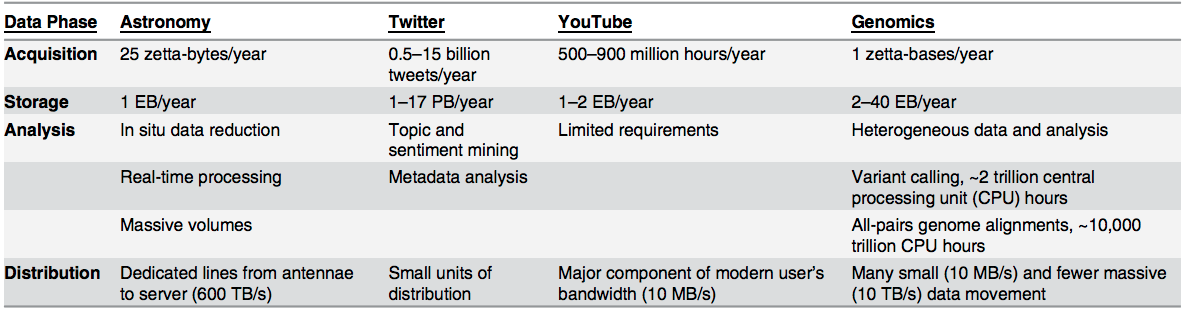
\includegraphics[width=\textwidth]{astrogeno}
  \caption{Projected annual storage and computing needs of four domains of Big Data in 2025. The phases of acquisition, storage, analysis, and distribution represent all the data lifecycle.}
  \label{fig:astrogeno}
\end{figure*}

\textbf{Story before.}
So the beautiful story that inspired our whole project starts with :
NEXT GENERATION SEQUENCING, a revolutionary set of technologies that make reading DNA very fast and not as expensive as it used to be In this way a huge number of genomic datases have been made available
How does it work specifically?
PRIMARY: Sequencing machines perform the primary data analysis  and produce raw datasets (a single human genome requires about 200 GB). 
SECONDARY: Computationally expensive pipelines, collectively regarded as secondary data analysis, are then applied to raw data for extracting signals from the genome (such as: mutations,
expression levels, peaks of binding enrichment, chromatin states, etc.), thereby producing processed genomic data , which are much smaller in size.
TERTIARY: Processed datasets are collected by worldwide consortia, such as TCGA (The Cancer Genome Atlas), ENCODE (the Encyclopedia of DNA Elements), …
Rough terms and sizes
\textit{Abstract Data}
The human DNA sequence is a string of 3.2 billions of base pairs, encoding adenine (A), cytosine (C), guanine (G), and thymine (T); size = 800Mbyte.
\textit{Raw/Aligned Data} 
Data is produced as «reads», overapping subportions of the genome, and then aligned to a reference genome, with empahsis on quality; size = 200GByte. 
\textit{Processed Data:}
But each of us has «just» 4.1M to 5M mutations, mostly single substitutions/insertions/deletions; size = 125Mbyte
We work on process data!!

WHich problems can we solve? (analysing process data)
Which cancer types can be explained by disregulation of the tri-dimensional structure of the genome?
Which co-occurring (killer) mutations cause the death of a cell in given tumors?
Which transcription factors (dimers) always occur together?
How can we assign predominant functions to each portion of the genome?

Our repository system aims at invogliare people to analyse data using our data model and out querying language






Research questions
Broader picture: Does the Bioinformatics community currently have a tool to locate 
interesting integrated data 
to solve biological/clinical questions?

Immediate scope: Wouldn’t the GMQL user be very happy with an integrated, semantically rich, repository to locate the right datasets 
for his/her research questions?



We want to:
-Focus on genomic open data; integration driven by a conceptual model
-Conceptual modeling for driving the continuous process of metadata integration and for locating relevant datasets
-Disclosure of the semantic properties of the sources; broader spectrum of sources covered, richer set of concepts provided
-Integration of subsets of these sources together

This work is included inside the bigger framework of GECO, an ERC advanced grant which aims to...

How would "experiments googling" help genomics researchers??
NIH sponsors donation and participation in Genomics Research, by providing precise non-discriminating policies on how to get involved, how personal privacy is protected, how study eligibility works for everyone\footnote{NIH maintains a portal for this ckind of information: \url{https://www.genome.gov/27561546/participating-in-genomics-research/}}.


\textbf{Paper organization.}




\section{The Genomic Conceptual Model}

Data integration (or information integration) is a set of techniques that allow heterogeneous data, coming from different sources, having various structures, formats, unities of measure, languages, to be uniformed into one global agreed representation.
Among other techniques, data integration can be based on the use of a \textit{conceptual model}, a composition of concepts which abstract a knowledge area in a compact shape, to make it more understandable and organized.



\section{The Integration Procedure}

\section{The Platform}

\section{Application in the Research Field}

Examples of biological problems

Given three replicas of a Chip.Seq experiment, extract high-confidence regions into one sample, identify which of these regions overlap with given genes, and for each resulting region count ICG mutations and select regions with at least one mutation.

3d structure and tumors

Same/cross gene activity correlations in normal vs tumor cells

Dimers: pairs of TFs that co-regulate genes in rigid and compact pairs.

Super-TADs: clusters of topological domains.

Killer Mutations: pairs of mutations: when both present they cause the death of the cell.

Identification of TFs that co-occur with TEAD4 binding sites.

Detect DNA areas where multiple TFs bind (dense TF binding regions).

DNA Sequencing of Microbioma in Cystic Fibrosis patients who are colonized with mycobacterium abscessus.

\begin{figure}
  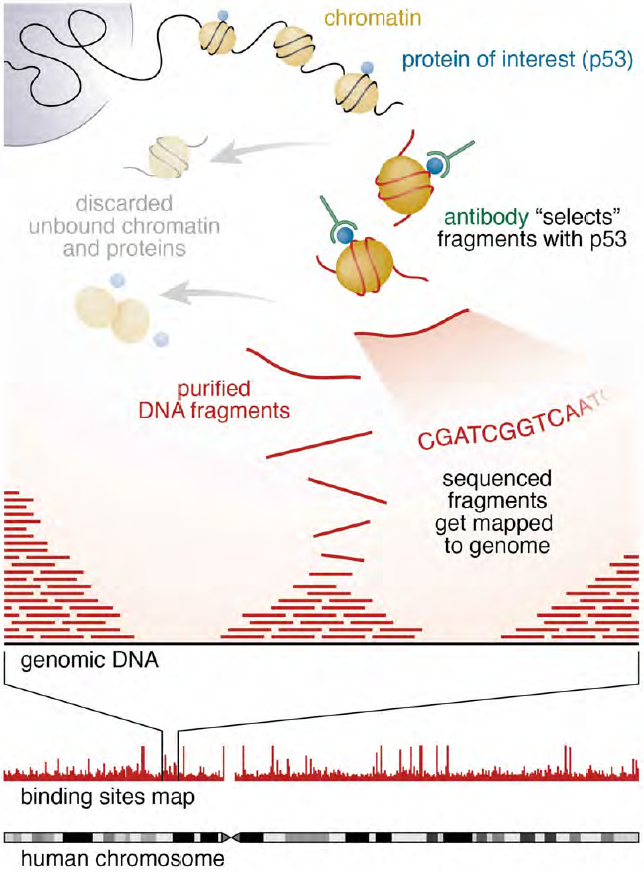
\includegraphics[width=\linewidth]{chip-seq_workflow}
  \caption{...}
  \label{fig:chipseq}
\end{figure}

\section{Related works.}
BioKleisli, K2, EnsMart/BioMart, BioStar \ldots provide integrated access to multiple, heterogeneous sources in the field of biomedical data;

Other works use conceptual models to explain biological entities and their interactions;

DeepBlue is an interesting starting point:  hiding of datasource differences to provide easy-to-use interfaces;

Big consortia efforts: BioProject database (from NCBI, EBI and DDBJ), Encode DCC (Data Coordination Center), Tcga GDC (Genomic Data Commons).


\section{Future Work and Conclusions}
We are delivering a repository, which will hopefully be appreciated by...


\cite{bernasconi2017conceptual}


prendere da http://www.bioinformatics.deib.polimi.it/geco/?home
e dal mio foglio di esame passaggio anno dottorato

{\bf Acknowledgment.} This research is funded by the ERC Advanced Grant project GeCo (Data-Driven Genomic Computing), 2016-2021.

\bibliographystyle{abbrv}
\bibliography{repo} 




\end{document}


